\subsection{Strategy}
\label{strategy}

\textbf{Scopo}: Comportamentale \\
\textbf{Raggio d'azione}: Oggetti

\paragraph{Definizione} Il pattern Strategy, a differenza di Template (\ref{template}), in cui si congela l'algoritmo per risolvere il problema a seconda del tipo di specifica, cambia l'algoritmo a seconda del tipo concreto. Ha lo scopo di definire una famiglia di algoritmi, incapsularli e renderli interscambiabili.

\begin{figure}[H]
    \centering
    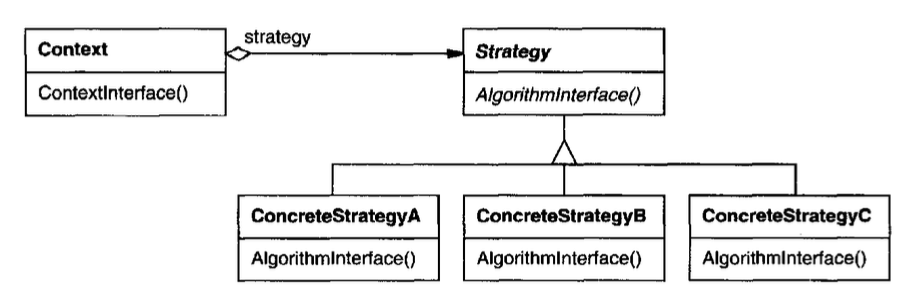
\includegraphics[width=0.5\linewidth]{assets/pattern/strategy/strategy-struttura.png}
    \caption{Struttura del pattern}
\end{figure}

\paragraph{Struttura e Conseguenze} Il pattern è composto da:
\begin{itemize}
    \item \textbf{Context}: mantiene un riferimento a una delle ConcreteStrategy e comunica con questo oggetto solo tramite l’interfaccia Strategy.
    \item \textbf{Strategy}: interfaccia comune a tutte le ConcreteStrategy. Dichiara un metodo che il contesto utilizza per eseguire una strategia.
    \item \textbf{ConcreteStrategy}: implementano diverse varianti di un algoritmo utilizzato dal Context.
    \item \textbf{Client}: crea un oggetto ConcreteStrategy e lo passa al Context, il quale espone un setter che consente ai Client di sostituire la Strategy associata al Context a runtime.
\end{itemize}

\paragraph{Applicabilità} Il pattern Strategy è utile quando si desidera utilizzare diverse varianti di un algoritmo all'interno di un oggetto ed essere in grado di passare da un algoritmo all'altro a runtime.

Risulta efficace quando si hanno molte classi simili che differiscono solo nel modo in cui eseguono alcuni comportamenti (queste classi spesso contengono istruzioni condizionali massicce per passare da un'algoritmo all'altro).

In più permette di isolare la logica di business di una classe dai dettagli di implementazione degli algoritmi che potrebbero non essere così importanti nel contesto di tale logica.

Può essere considerato come un'estensione del pattern State (\ref{state}), entrambi sono basati sulla \textbf{composizione}: modificano il comportamento del contesto delegando parte del lavoro agli oggetti helper. Sebbene, il pattern State non limiti le dipendenze tra stati concreti, consentendo loro di alterare a piacimento lo stato del contesto.

\begin{figure}[H]
    \centering
    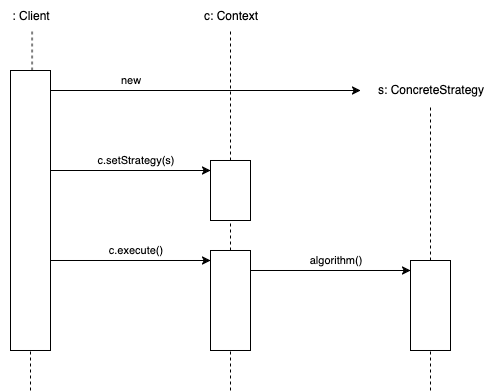
\includegraphics[width=0.7\linewidth]{assets/pattern/strategy/strategy-sequence.drawio.png}
\end{figure}

\paragraph{Vantaggi}
\begin{itemize}
    \item È possibile scambiare gli algoritmi utilizzati all'interno di un oggetto in fase di esecuzione.
    \item È possibile isolare i dettagli di implementazione di un algoritmo dal codice che lo utilizza.
    \item Si possono introdurre nuove strategie senza dover modificare il contesto.
\end{itemize}

\paragraph{Svantaggi}
\begin{itemize}
    \item I client devono essere consapevoli delle differenze tra le strategie per poter selezionare quella più adeguata.
    \item Se si hanno solo un paio di algoritmi che cambiano raramente, l'uso del pattern può introdurre complessità non necessaria con nuove classi e interfacce.
\end{itemize}


\newpage